We compare our custom pairwise tensor contraction algorithm to the einsum engines of PyTorch and Numpy as well as with the np\_mm backend. To evaluate the performance of each engine, we us two different sets of problems: First, we test all four engines on simple pairwise tensor contractions with different structural characteristics. Second, we evaluate the four einsum engines on real-world einsum expressions.\\
\textcite{blacher2024einsum} point out that most current tensor libraries are optimized for a limited range of tensor operations, particularly those involving large, dense tensors. However, real-world applications often require a much broader variety of tensor operations, which can cause performance issues. To solve this problem, they present the einsum\_benchmark dataset that includes a wide range of tensor operations and covers the diverse types of operations used in practice. To address this issue, we assesse the performance of all four different implementations on 28 real-world problems from that dataset.\\
We measure the iterations per second for all experiments, that is, how often a given einsum expression can be executed within one second. The experiments are performed on a machine with
an Intel i5-7200U 2-core processor running Ubuntu 22.04-1 with 8 GB of RAM.
Each core has a base frequency of 2.5 GHz and a max boost frequency of 3.1 GHz. The evaluation is done in
Python 3.12.8 with PyTorch 2.5.1 and Numpy 2.2.1.

\section{Experiments on Pairwise Tensor Contractions}
We designed four format strings for pairwise tensor contractions with or without batch dimensions, traces and arbitrary indices in different combinations as can be seen in Table \ref{tab:instance:data}.
\begin{table}[H]
    \caption{Format string and properties of the four einsum expressions.}
    \label{tab:instance:data}
    \centering
    { % Apply the scriptsize font to the entire table
    \begin{tabularx}{\textwidth}{>
    {\raggedright\arraybackslash}p{3cm} >
    {\centering\arraybackslash}X >
    {\centering\arraybackslash}X >
    {\centering\arraybackslash}X}
        \toprule
        \textbf{einsumstring} & \textbf{batch dim} & \textbf{traces} & \textbf{arbitrary indices} \\
        \midrule
        aabcd,adeef$\rightarrow$dcf & yes & yes & yes  \\
        abcd,adef$\rightarrow$dbef & yes & no & yes  \\
        aabcd,adeef$\rightarrow$bcf & no  & yes & yes  \\
        abcd,adef$\rightarrow$cbef & no  & no  & no   \\
        \bottomrule
    \end{tabularx}
    }
\end{table}

\noindent In order to test the performance of the four einsum engines across scenarios with increasing compute intensity, we generated random tensors for each problem several times, each time with bigger dimensions. For example, the first pair of tensor we created for the einsum expression aabcd,adeef$\rightarrow$dcf had sizes (2,2,2,2,2) for both tensor $A$ and $B$, resulting in 128 floating point operations (or 2.11 floating point operations if we use a log10 scale). A table with the dimension sizes and resulting floating point operations for the four problems can ba found in Table~\ref{tab:dimensions} in the appendix.\\

\noindent As can be seen in Figure~\ref{flops}, our custom implementation outperformes PyTorch and Numpy for problems that contain batch dimensions, traces and arbitrary indices.
\begin{figure}[h]
    \label{flops}
    \centering
    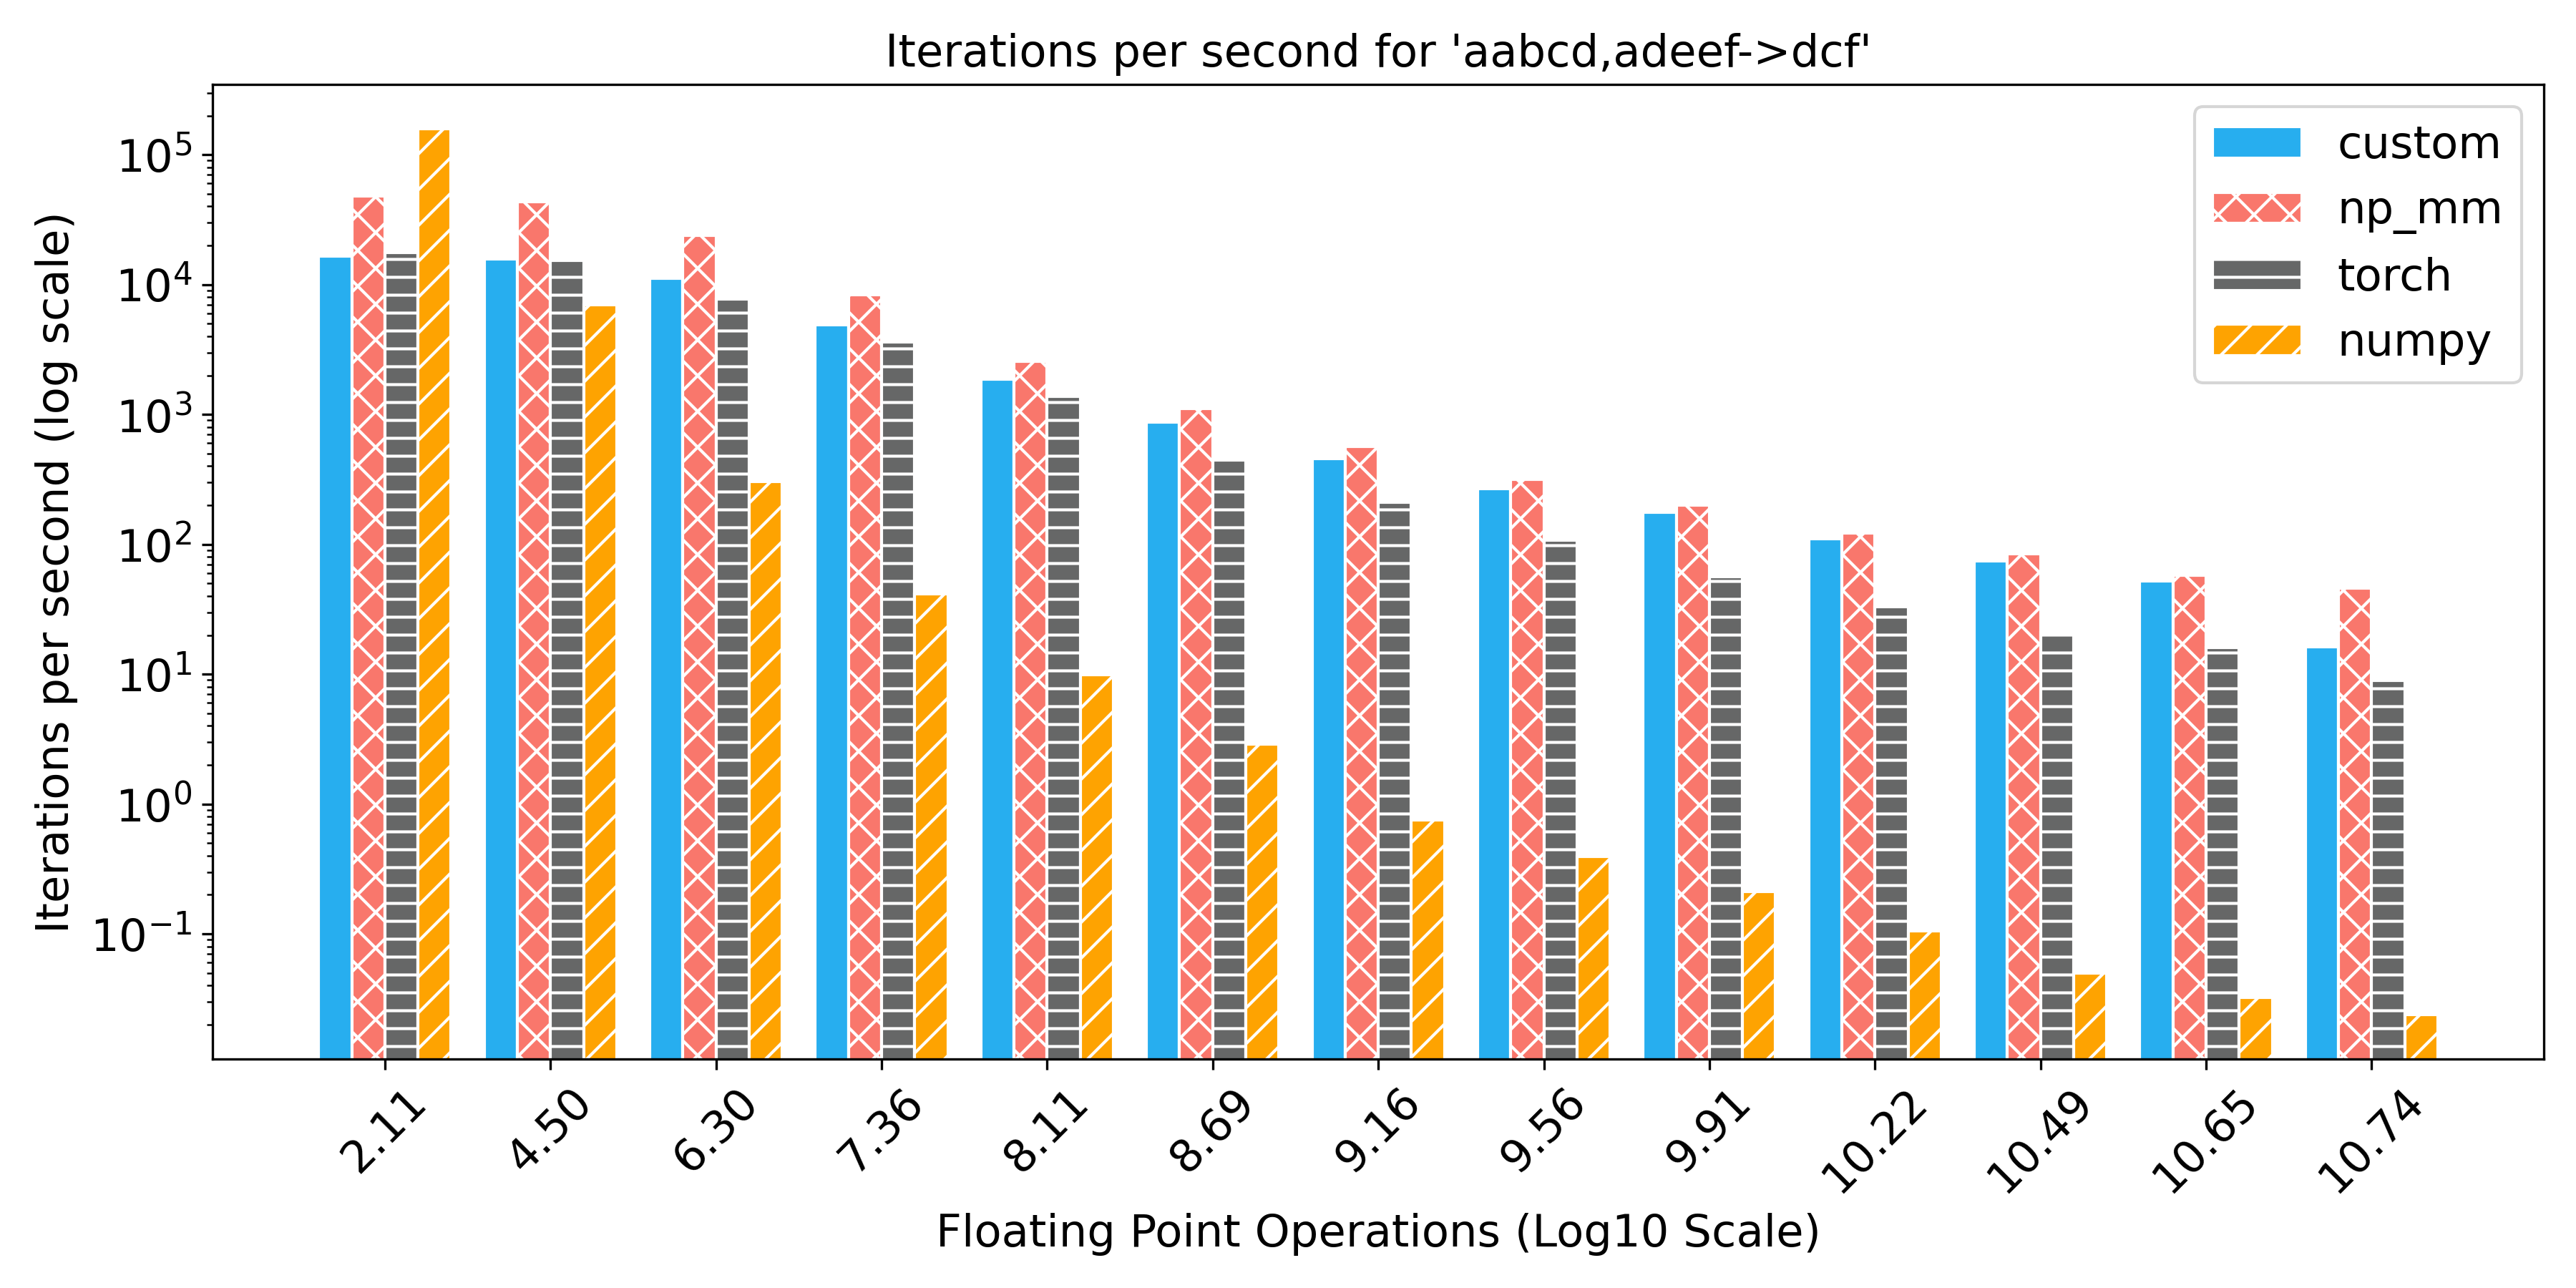
\includegraphics[width=1\textwidth]{images/aabcd_adeef__dcf.png}  % Include your image
    \caption{Performance Comparison for a problem with batch dimensions, traces and arbitrary indices. The x-axis depicts the number of floating point operations corresponding to the gradually increased dimension sizes.}
\end{figure}

\noindent While the performance of all implementations decreases with a growing number of floating-point operations over all four problems, the rate of this degration varies. Numpy performs better than all the other backends for low counts of floating-point operations in all four contractions, as can be seen in Figure~\ref{pic:all}. However, its performance declines fastly with increasing problem size. For the largest problems, our algorithm with the np\_mm backend emerges as the most efficient method across all cases, as can be seen in Table~\ref{tab:flop_comp}.

\begin{table}[H]
    \caption{Performance comparison for the largest tensor contractions of the respective problems across the different engines.}
    \label{tab:flop_comp}
    \centering
    {\scriptsize  % Apply the scriptsize font to the entire table
    \begin{tabularx}{\textwidth}{>
    {\raggedright\arraybackslash}p{4cm} >
    {\centering\arraybackslash}X >
    {\centering\arraybackslash}X >
    {\centering\arraybackslash}X >
    {\centering\arraybackslash}X >
    {\centering\arraybackslash}X}
        \toprule
        \textbf{\scriptsize Tensor Expression} & \textbf{\scriptsize FLOPS}\textbf{\scriptsize Custom} & \textbf{\scriptsize np\_mm} & \textbf{\scriptsize Numpy} & \textbf{\scriptsize Torch} \\
        \midrule
        aabcd,adeef$\rightarrow$dcf &10.74& 0.35 &\textbf{ 1} & 0.00043 & 0.19 \\
        abcd,adef$\rightarrow$dbef &10.93& 0.36 &\textbf{ 1} & 0.0014  & 0.72 \\
        aabcd,adeef$\rightarrow$bcf &10.74& 0.15 &\textbf{ 1} & 0.001   & 0.42 \\
        abcd,adef$\rightarrow$cbef &10.93& 0.11 &\textbf{ 1} & 0.03    & 0.98 \\
        \bottomrule
    \end{tabularx}
    }
\end{table}


\section{Einsum Benchmark} 
\begin{figure}[H]
    \centering
    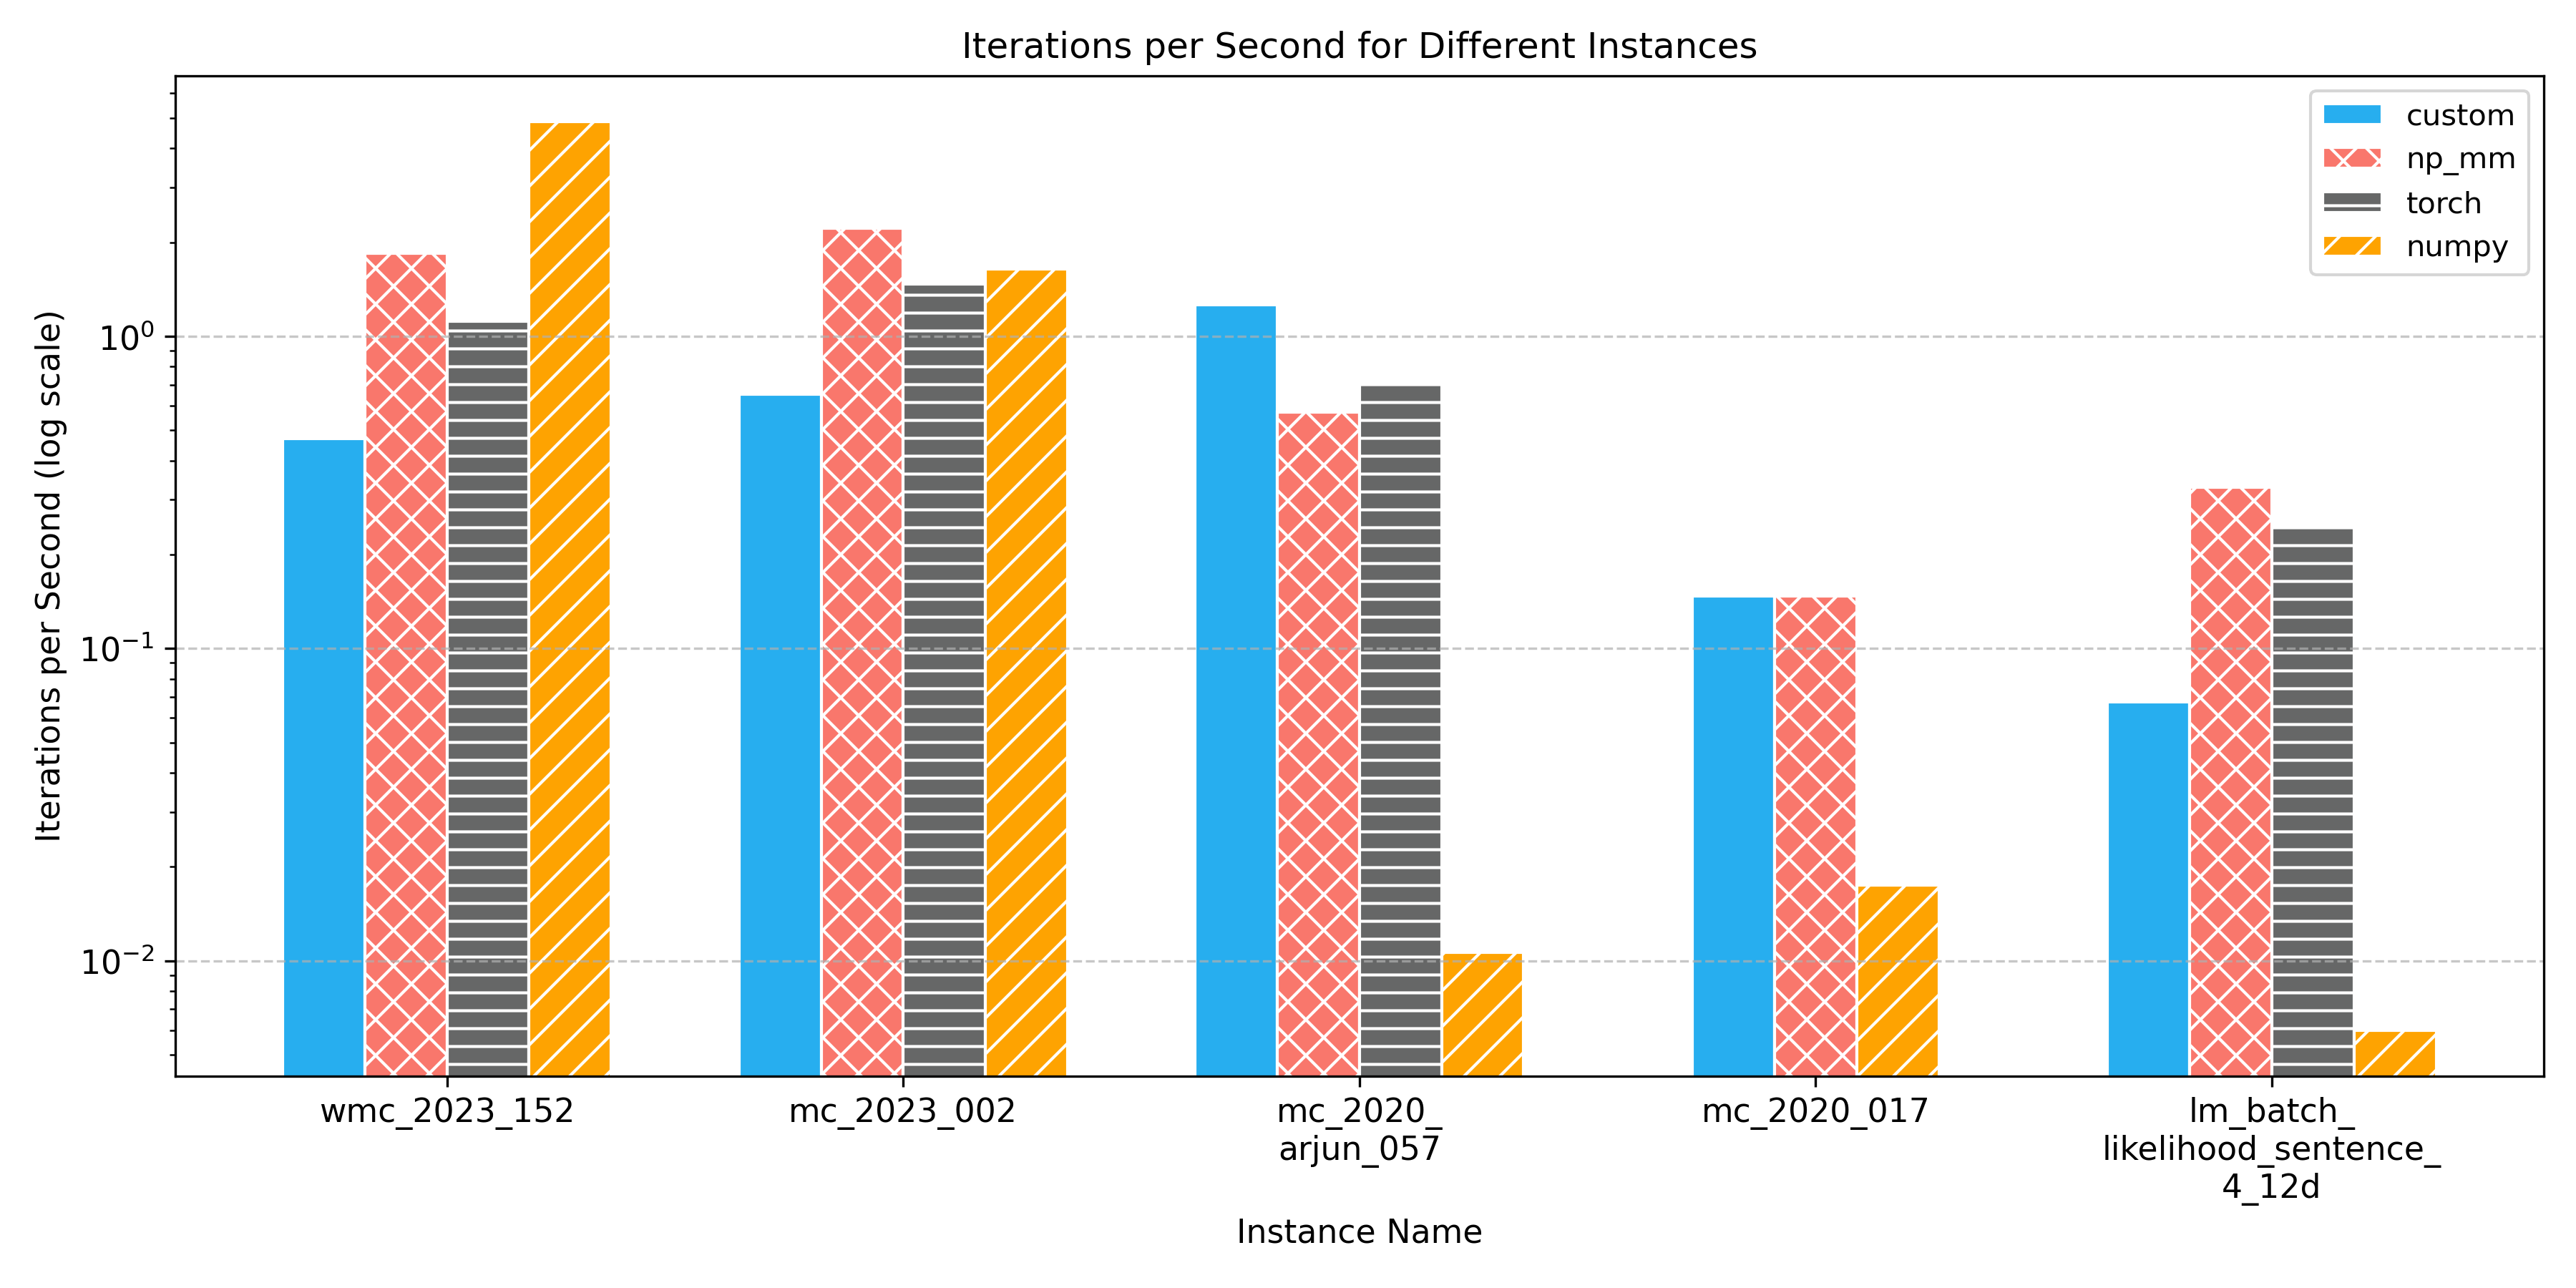
\includegraphics[width=1\textwidth]{images/einsum_five.png} 
    \caption{Performance Comparison for different problems from einsum\_benchmark~\cite{blacher2024einsum}.}
    \label{e_b}
\end{figure}
We ran the 28 problems from the einsum\_benchmark dataset~\cite{blacher2024einsum} that are small enough to fit on our machine and have a non-complex data type. For our performance discussion we chose representative problems that depict the differences between the four einsum engines. Table \ref{tab:properties} lists the relevant properties of these problems.
\begin{table}[H]
    \caption{Instance data with instance name, number of tensors and the size of the biggest intermediate tensor.}
    \label{tab:properties}
    \centering
    {\scriptsize  % Apply the scriptsize font to the entire table
    \begin{tabularx}{\textwidth}{>
    {\raggedright\arraybackslash}p{4cm} >
    {\centering\arraybackslash}X >
    {\centering\arraybackslash}X}
        \toprule
        \textbf{\scriptsize Instance Name} & \textbf{\scriptsize Number of Tensors} & \textbf{\scriptsize Biggest Intermediate Tensor} \\
        \midrule
        wmc\_2023\_152 & 40489 & 16384 \\
        mc\_2023\_002  & 26556 & 131072 \\
        mc\_2020\_arjun\_057 & 905 & 8388608 \\
        lm\_batch\_likelihood\_sentence\_4\_12d & 84 & 39398400 \\
        mc\_2020\_017  & 78784 & 4194304 \\
        \bottomrule
    \end{tabularx}
    }
\end{table}
\sloppy
\noindent As shown in Figure \ref{e_b}, Numpy performs best for problems with small intermediate tensor sizes. Our custom algorithm is more efficient for problems involving the int data type, while PyTorch outperforms both our algorithm and the custom np\_mm BMM for problems with the double data type.\\
Casting the instances data type from int\_32 to float\_64, we found that the performance of our custom algorithm remained unchanged, while PyTorch and np\_mm saw significant improvements, outperforming our algorithm. Here, the np\_mm implementation performed better than PyTorch on the instance lm\_batch\_likelihood\_sentence\_4\_12d.


\section{Impact of Parallelization}
\begin{figure}[H]
    \centering
    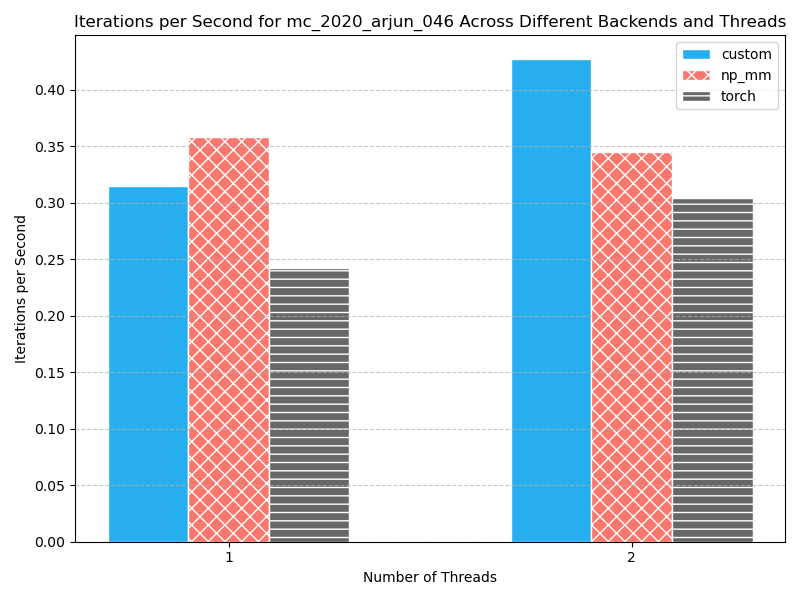
\includegraphics[width=0.6\textwidth]{images/threads.png}  % Include your image
    \caption{Iterations per second vs thread number for mc\_2020\_arjun\_046~\cite{blacher2024einsum}.}
    \label{threads}
\end{figure}
\noindent We evaluated a multi-tensor contraction using our custom implementation, our implementation with the np\_mm backend, and PyTorch on one and two threads. While NumPy’s batch matrix multiplication is not parallelized, our custom multi-tensor contraction showed an approximate 25\% performance improvement when increasing the thread count from one to two. PyTorch’s performance similarly improved by around 20\%. Additionally, we measured the isolated performance of our custom BMM computation. Here, the parallelization lead to an almost 50\% speed-up when scaling from one to two threads. 
